\section{Rechnungsbsp}
\subsection{B2U RC}
\begin{minipage}{0.4\linewidth}
    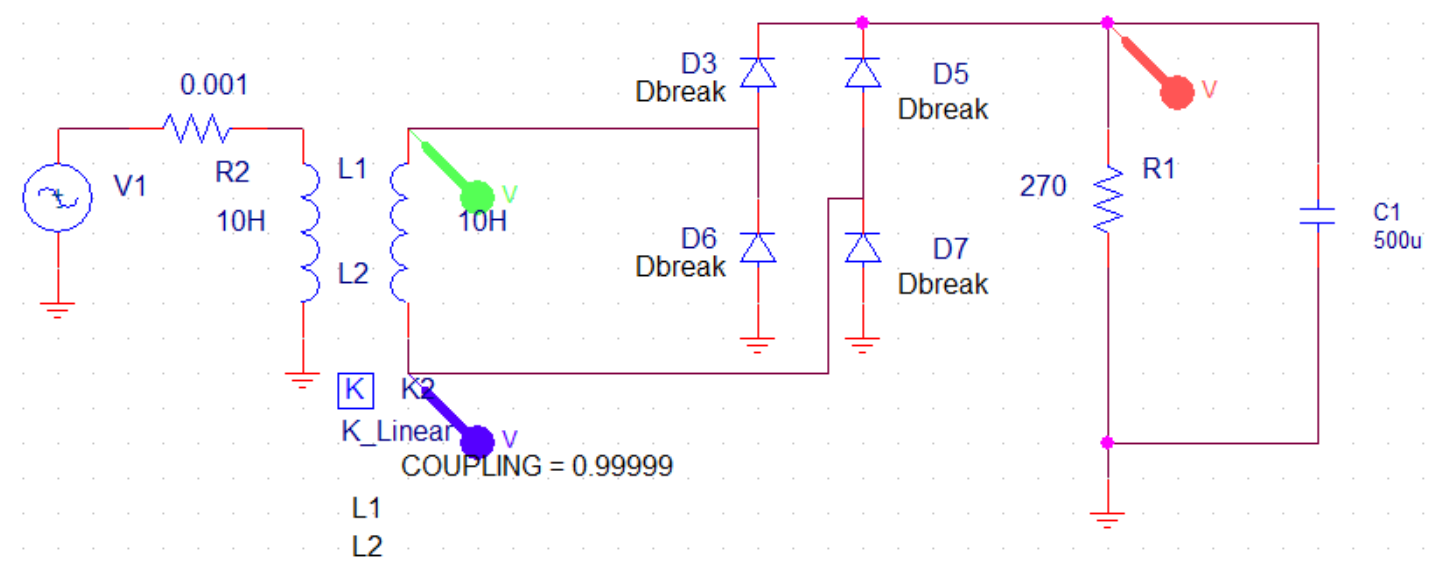
\includegraphics[width=\linewidth]{images/Rechnungsbsp/B2URC}
\end{minipage}
\begin{minipage}{0.2\linewidth}
    \includegraphics[width=\linewidth]{images/Rechnungsbsp/B2URCKl}
\end{minipage}
\begin{minipage}{5cm}
   $ R = 270 $ \newline
   $ C = 500 \cdot 10^{-6} $\newline
   $ U_{2m} = 30 $ \newline
   $ f = 50 Hz $   
\end{minipage}
\newline
\textbf{Diode Sperrt:} $ U_R > U_2 \quad \rightarrow \quad $ Sperrwinkel $\alpha$ $\qquad \alpha \leq \beta \leq \gamma$
\begin{align*}
     0 & = i_R + i_C \\
     0 & = \frac{U_R}{R}+ C \frac{\diff U_R}{\diff t} \qquad \tau = RC \qquad t = \frac{\beta}{\omega}\\
     - \frac{t}{\tau} + A & = \frac{1}{U_R} \diff U_R \\
     U_R(\beta) & = B \cdot e^{-\frac{\beta}{\omega \tau}}
     \end{align*}
 Um B herauszufinden müssen die Anfangsbedingungen eingesetzt werden.\newline 
 Beim Winkel $\alpha$ ist der Spg-Verlauf von $U_2$ = der StartSpg. 
     \begin{align*}
     U_R(\alpha) & =U_R(\alpha)\\
     U_{2m} \cdot sin(\alpha) & = B \cdot e^{-\frac{\alpha}{\omega \tau}}\\
     B & = U_{2m} \cdot sin(\alpha) \cdot e^{\frac{\alpha}{\omega \tau}}\\
     U_R(\beta) & =  U_{2m} \cdot sin(\alpha) \cdot e^{-\frac{\beta - \alpha}{\omega \tau}} \qquad \alpha \leq \beta \leq \gamma       
\end{align*}
Als nächstes müssen wir $\alpha$ bestimmen. Sobald die Steigung von $U_R \neq U_{2}$ sperrt die Diode $\alpha = \beta$
\begin{align*}
    U_R(\beta) \frac{\diff}{\diff \beta} & = U_2(\beta) \frac{\diff}{\diff \beta}\\
    \left( U_{2m} \cdot sin(\alpha) \cdot e^{-\frac{\beta - \alpha}{\omega \tau}}\right)\frac{\diff}{\diff \beta} & = \left( U_{2m} \cdot sin(\beta)\right)\frac{\diff}{\diff \beta}\\
    U_{2m}\cdot sin(\alpha)\cdot e^{\frac{\alpha - \beta}{\omega \tau}}\cdot \frac{-1}{\omega \tau} &= U_{2m}\cdot cos(\beta) \qquad | \alpha = \beta\\
    sin(\alpha)\cdot \frac{-1}{\omega \tau} &= cos(\alpha)\\
    \alpha & = -arctan(\omega \tau) \qquad 0 < \alpha < \pi\\
    \alpha & = -1.547 \qquad \pi -Periodisch\\
    \alpha & = 1.5943 \rightarrow 91.35_{grad}
\end{align*}

\textbf{Diode leitet:} $ U_R < U_2 \quad \rightarrow \quad $ Durchlasswinkel $\gamma \qquad \gamma \leq \beta \leq \alpha$
\begin{align*}
    U_2(\gamma) & = U_R(\gamma)\\
    U_{2m}\cdot -sin(\gamma) & = U_{2m} \cdot sin(\alpha) \cdot e^{-\frac{\gamma - \alpha}{\omega \tau}}\\
    -sin(\gamma) & = sin(\alpha) \cdot e^{\frac{\alpha - \gamma}{\omega \tau}} \qquad \pi < \gamma < \nicefrac{3\pi}{2}\\
    \gamma & = 4.354 \rightarrow 249.5_{grad}
\end{align*}

\textbf{Diode leitet} $ \gamma - \pi = 69_{grad} < \beta < \alpha = 91.35_{grad} $\newline
\[  U_R(\beta) = U_{2m} \cdot sin(\beta)\]

\textbf{Diode sperrt} $ \alpha = 91.35_{grad}< \beta < \gamma = 249.5_{grad}  $\newline
\[  U_R(\beta)  =  U_{2m} \cdot sin(\alpha) \cdot e^{-\frac{\beta - \alpha}{\omega \tau}}\]

%=============================================================
\clearpage
\subsection{M1U RL}
\begin{minipage}{0.4\linewidth}
    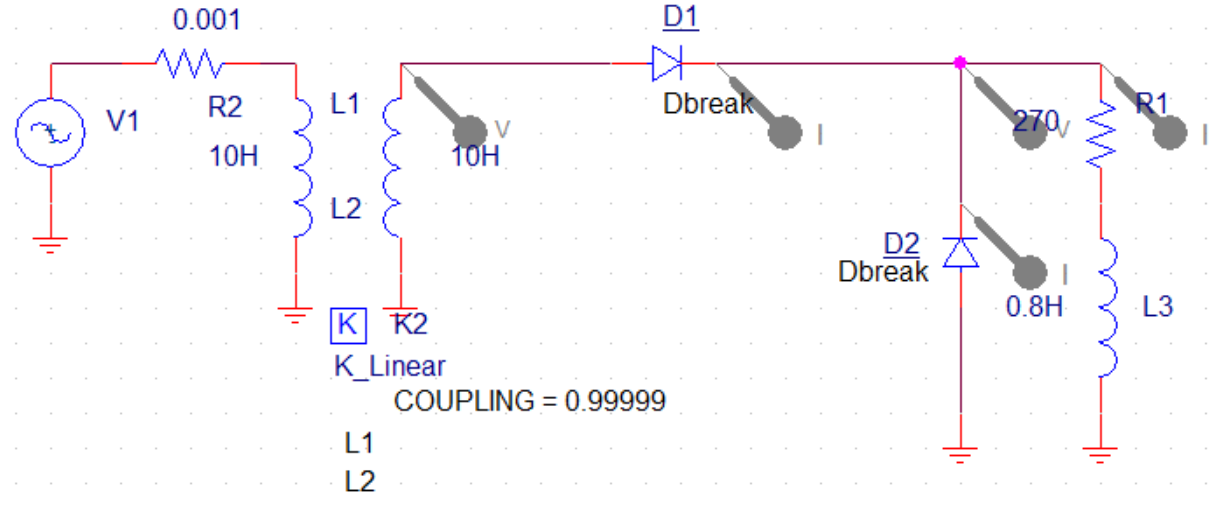
\includegraphics[width=\linewidth]{images/Rechnungsbsp/M1URL}
\end{minipage}
\begin{minipage}{0.2\linewidth}
    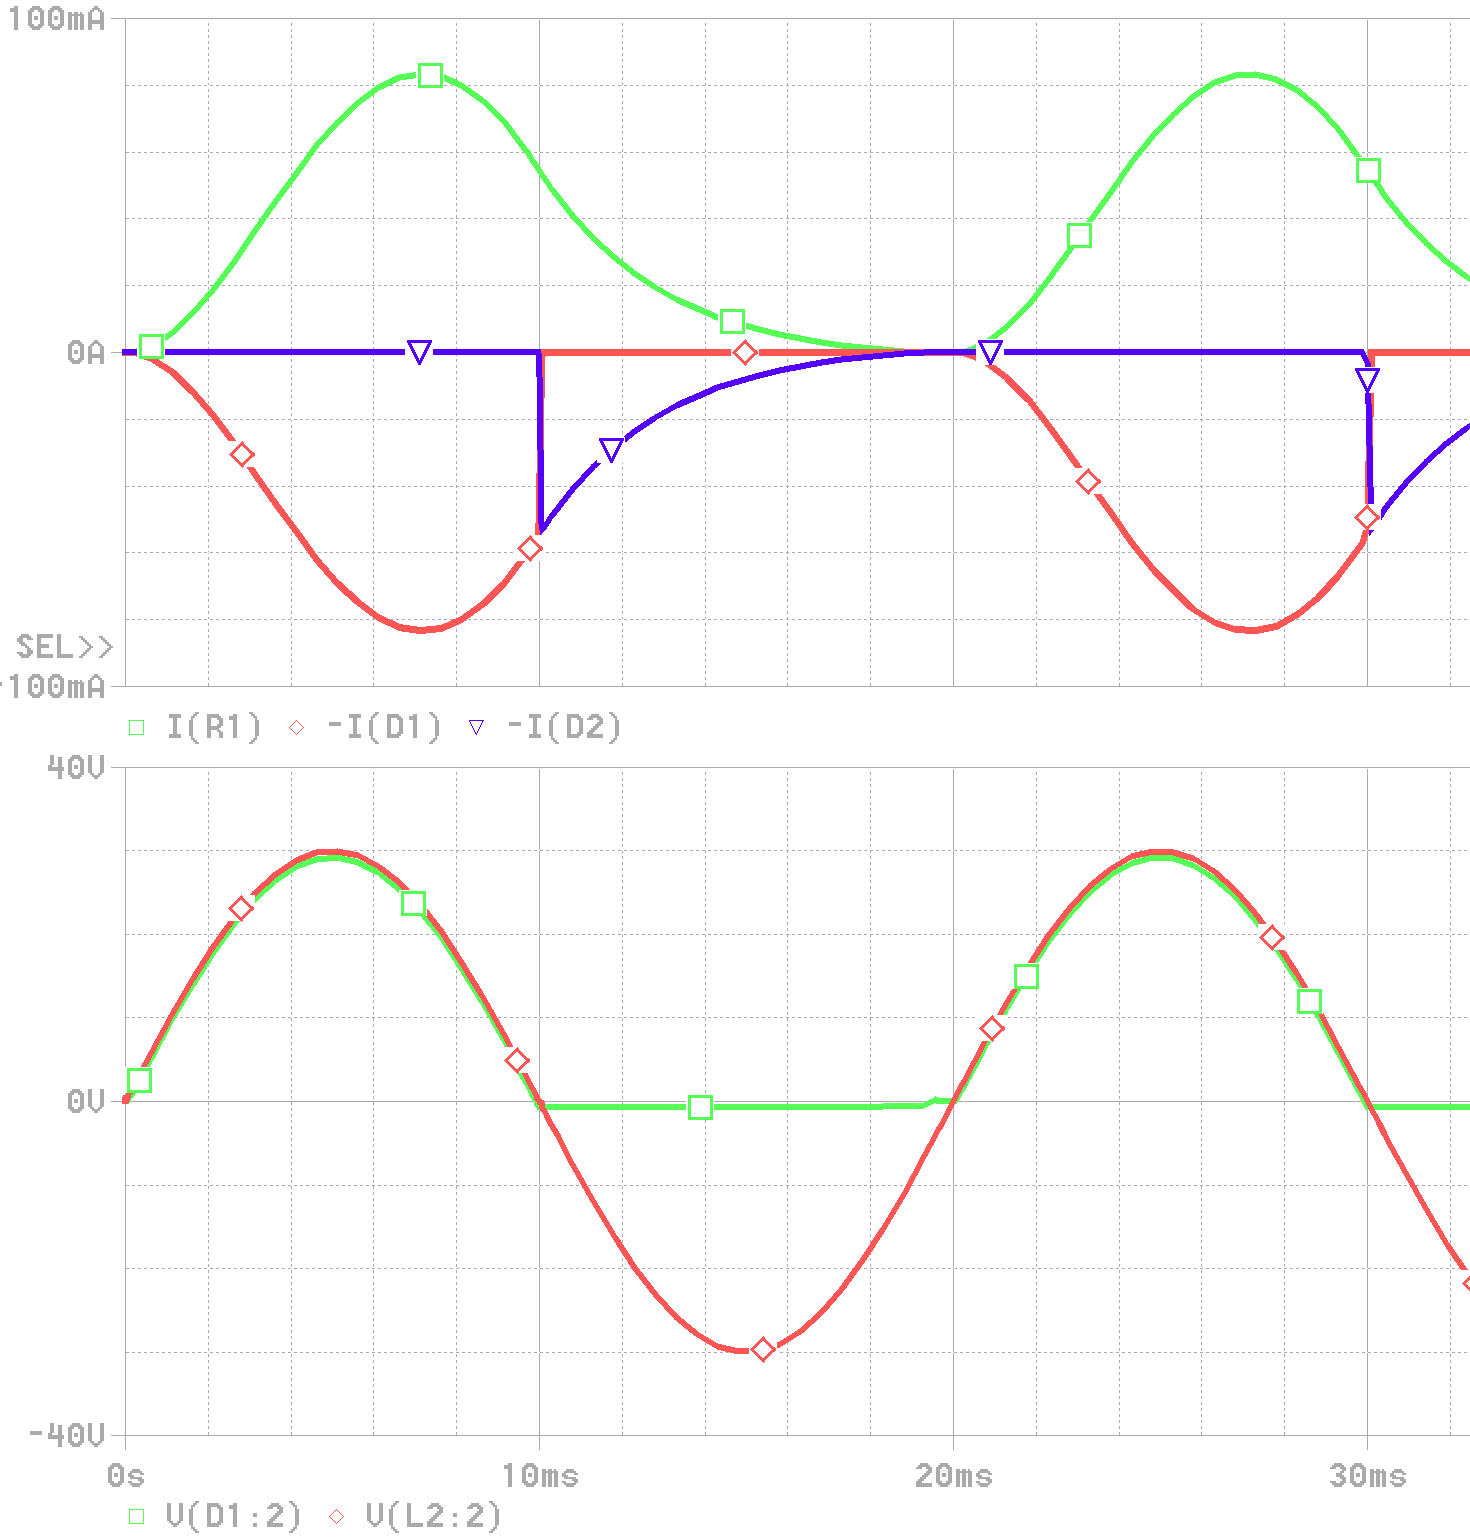
\includegraphics[width=\linewidth]{images/Rechnungsbsp/M1URLKL}
\end{minipage}
\begin{minipage}{5cm}
    $ R = 270 $ \newline
    $ C = 500 \cdot 10^{-6} $\newline
    $ U_{2m} = 30 $ \newline
    $ f = 50 Hz $   
\end{minipage}

\textbf{Diode leitet:} $ 0 < t < \pi falsch $ $ 0 \leq \beta \leq \pi $\newline
$U_2(t) = i_R + L\frac{\diff i(t)}{\diff t}$\newline
\textbf{Homogen Lösung}
\begin{align*}
     0 = & i_R + L \frac{\diff i(t)}{\diff t} \\
     i_{h1} = & C_2 \cdot e^{\frac{-t}{\tau}} = C_2 \cdot e^{\frac{-\beta}{\omega \tau}}
\end{align*} 

\textbf{partikuläre Lösung}
\begin{align*}
    U_{2m}\cdot sin(\omega t) = & R\cdot i_{p1} + L \frac{\diff i_{p1}}{\diff t}\\
    k \cdot sin(b \cdot x)= & A \cdot cos(b \cdot x) + B \cdot sin(b \cdot x) \qquad \text{Ansatz Störglied}\\
    i_{p1} = & A \cdot cos(\omega t) + B \cdot sin(\omega t)\\
    \frac{\diff i_{p1}}{\diff t} = & - A \cdot \omega \cdot sin(\omega t) + B \cdot \omega \cdot cos(\omega t)\\
    U_{2m}\cdot sin(\omega t) = & R\cdot A \cdot cos(\omega t) + R\cdot B \cdot sin(\omega t)  - L\cdot A \cdot \omega cos(\omega t) + L\cdot B \cdot \omega \cdot cos(\omega t)\\
    U_{2m}\cdot sin(\omega t) + 0\cdot cos(\omega t) = & sin(\omega t)(R \cdot B - L \cdot \omega \cdot A) + cos(\omega t)(R\cdot A + L \cdot \omega \cdot  A)
\end{align*}
\begin{minipage}{5cm}
    $rref
    \begin{bmatrix}
    -L\omega       &R  & U_{2m} \\ 
    R&L\omega          & 0
    \end{bmatrix} 
    \rightarrow$ 
\end{minipage}
\begin{minipage}{5cm}
    \[ A = -U_{2m} \frac{L\omega}{R^2 + L^2\omega^2} \]
    \[ B = U_{2m} \frac{R}{R^2 + L^2\omega^2} \]
\end{minipage}
\begin{align*}
    i_1 = & i_{p1} + i_{h1}\\
    i_{p1} = & \frac{U_{2m}}{R^2 + L^2\omega^2}\left(sin(\omega t) R - cos(\omega t) L\omega\right)\\
    i_{h1} = & C_2 \cdot e^{\frac{-t}{\tau}}\\
    i_{1}(\beta) = & \frac{U_{2m}}{R^2 + L^2\omega^2}\left(sin(\beta) R - cos(\beta) L\omega\right) + C_2 \cdot e^{\frac{-\beta}{\omega \tau}}
\end{align*}

\textbf{Diode sperrt:}$ \pi \leq \beta \leq 2\pi$\newline
$0 = i_R + L\frac{\diff i(t)}{\diff t}$\newline
\textbf{Homogen Lösung}
\begin{align*}
i_{h2} = & C_3 \cdot e^{\frac{-t}{\tau}} = C_3 \cdot e^{\frac{-\beta}{\omega \tau}}\\
i_2(\beta) = & i_{h2}
\end{align*}
\\
\textbf{Anfangsbedingungen}
\begin{align*}
    i_1(\pi) = & i_2(\pi)\\
    i_1(0)  = & i_2(2\pi)
\end{align*}

\textbf{Ströme vergleichen}
\begin{align*}
    \beta = \pi \qquad & \qquad \beta = \pi\\
    - U_{2m} \frac{L\omega}{R^2 + L^2\omega^2} + C_2 \cdot e^{\frac{-\pi}{\omega \tau}} = & C_3 \cdot e^{\frac{-\pi}{\omega \tau}}\\
    \beta = 0 \qquad & \qquad \beta = 2\pi\\
    U_{2m} \frac{L\omega}{R^2 + L^2\omega^2} + C_2  = & C_3 \cdot e^{\frac{-2\pi}{\omega \tau}}\\  
\end{align*}
\begin{minipage}{7cm}
    $rref
    \begin{bmatrix}
    e^{\frac{-\pi}{\omega \tau}}       &-e^{\frac{-\pi}{\omega \tau}}  & U_{2m} \frac{L\omega}{R^2 + L^2\omega^2} \\ 
    1& -e^{\frac{-2\pi}{\omega \tau}}         & -U_{2m} \frac{L\omega}{R^2 + L^2\omega^2}
    \end{bmatrix} 
    \rightarrow$ 
\end{minipage}
\begin{minipage}{5cm}
    \[ C_2 = U_{2m} \frac{L \cdot \omega}{R^2 + L^2\omega^2} \cdot  \frac{e^{\frac{\pi}{\omega \tau}}}{e^{\frac{\pi}{\omega \tau}} +1} \]
    \[ C_3 = -U_{2m} \frac{L \cdot \omega}{R^2 + L^2\omega^2} \cdot  \frac{e^{\frac{2\pi}{\omega \tau}}}{e^{\frac{\pi}{\omega \tau}} +1} \]
\end{minipage}
\\
\textbf{Diode Leitet} $ 0 \leq \beta \leq \pi $\newline
\[ i_{1}(\beta) =  U_{2m} sin(\beta) \frac{R}{R^2 + L^2\omega^2} - U_{2m} cos(\beta) \frac{L \cdot \omega}{R^2 + L^2\omega^2} + U_{2m} \frac{L \cdot \omega}{R^2 + L^2\omega^2} \cdot  \frac{e^{\frac{\pi}{\omega \tau}}}{e^{\frac{\pi}{\omega \tau}} +1} \cdot e^{\frac{-\beta}{\omega \tau}} \]

\textbf{Diode Sperrt} $ \pi \leq \beta \leq 2\pi $\newline
\[ i_2(\beta) = -U_{2m} \frac{L \cdot \omega}{R^2 + L^2\omega^2} \cdot  \frac{e^{\frac{2\pi}{\omega \tau}}}{e^{\frac{\pi}{\omega \tau}} +1} \cdot e^{\frac{-\beta}{\omega \tau}} \]
\clearpage












